\documentclass[11pt]{article}

\usepackage[margin=1in]{geometry}
\usepackage[T1]{fontenc}
\usepackage[utf8]{inputenc}
\usepackage{lmodern}
\usepackage{microtype}
\usepackage{amsmath,amssymb,amsthm,mathtools,bm}
\usepackage{booktabs,array,tabularx,longtable}
\usepackage{enumitem}
\usepackage{xcolor}
\usepackage{hyperref}
\usepackage{tikz}
\usepackage{pgfplots}
\usepackage{tikz-3dplot}
\usepackage[most]{tcolorbox}
\usepackage{caption}
\usepackage{float}
\usepackage{fancyhdr}
\usepackage{titlesec}
\usepackage{listings}

\pgfplotsset{compat=1.18}
\usetikzlibrary{arrows.meta,calc,positioning,decorations.pathreplacing,patterns,fit,shapes.geometric,matrix,backgrounds,3d}

\definecolor{chapterblue}{HTML}{1F5AA6}
\definecolor{chapterteal}{HTML}{168A8F}
\definecolor{chapterorange}{HTML}{D9822B}
\definecolor{chaptergreen}{HTML}{2D8A4E}
\definecolor{chapterpurple}{HTML}{6B4EAA}
\definecolor{chapterred}{HTML}{B23B3B}
\definecolor{softblue}{HTML}{EAF3FF}
\definecolor{softgreen}{HTML}{EAF8EF}
\definecolor{softorange}{HTML}{FFF4E6}
\definecolor{softpurple}{HTML}{F3EEFF}
\definecolor{softred}{HTML}{FFF0F0}
\definecolor{softgray}{HTML}{F6F7F9}
\definecolor{darkgray}{HTML}{30343B}

\hypersetup{
  colorlinks=true,
  linkcolor=chapterblue,
  urlcolor=chapterblue,
  citecolor=chapterblue,
  pdftitle={Chapter 27 Review Synthesis and Bridge to Graduate Study}
}

\setlength{\parindent}{0pt}
\setlength{\parskip}{0.64em}
\setlength{\headheight}{14pt}
\setlist[itemize]{topsep=2pt,itemsep=2pt,leftmargin=1.5em}
\setlist[enumerate]{topsep=2pt,itemsep=2pt,leftmargin=1.7em}

\pagestyle{fancy}
\fancyhf{}
\lhead{Chapter 27. Review, Synthesis, and Bridge to Graduate Study}
\rhead{\thepage}
\renewcommand{\headrulewidth}{0.4pt}

\titleformat{\section}{\Large\bfseries\color{chapterblue}}{}{0em}{}
\titleformat{\subsection}{\large\bfseries\color{darkgray}}{}{0em}{}
\titleformat{\subsubsection}{\normalsize\bfseries\color{darkgray}}{}{0em}{}

\newcommand{\R}{\mathbb R}
\newcommand{\grad}{\nabla}
\newcommand{\dd}{\,d}
\newcommand{\norm}[1]{\left\lVert #1\right\rVert}
\newcommand{\inner}[2]{#1\cdot #2}
\newcommand{\proj}{\operatorname{proj}}
\newcommand{\diver}{\operatorname{div}}
\newcommand{\curl}{\operatorname{curl}}

\newtcolorbox{chapteroverviewbox}{
  enhanced,breakable,
  colback=softblue,
  colframe=chapterblue,
  boxrule=0.7pt,
  arc=2mm,
  left=2mm,right=2mm,top=1mm,bottom=1mm
}
\newtcolorbox{goalbox}{
  enhanced,breakable,
  colback=softgreen,
  colframe=chaptergreen,
  title=Learning goals,
  fonttitle=\bfseries,
  boxrule=0.7pt,
  arc=2mm
}
\newtcolorbox{tipbox}[1][]{
  enhanced,breakable,
  colback=softgreen,
  colframe=chaptergreen,
  title=#1,
  fonttitle=\bfseries,
  boxrule=0.7pt,
  arc=2mm
}
\newtcolorbox{warningbox}[1][]{
  enhanced,breakable,
  colback=softorange,
  colframe=chapterorange,
  title=#1,
  fonttitle=\bfseries,
  boxrule=0.7pt,
  arc=2mm
}
\newtcolorbox{summarybox}[1][]{
  enhanced,breakable,
  colback=softpurple,
  colframe=chapterpurple,
  title=#1,
  fonttitle=\bfseries,
  boxrule=0.7pt,
  arc=2mm
}
\newtcolorbox{examplebox}[1][]{
  enhanced,breakable,
  colback=white,
  colframe=chapterblue,
  title=#1,
  fonttitle=\bfseries,
  boxrule=0.7pt,
  arc=2mm
}
\newtcolorbox{formulabox}[1][]{
  enhanced,breakable,
  colback=softgray,
  colframe=darkgray!60,
  title=#1,
  fonttitle=\bfseries,
  boxrule=0.6pt,
  arc=2mm
}

\lstdefinestyle{pythonstyle}{
  basicstyle=\ttfamily\small,
  keywordstyle=\color{chapterblue}\bfseries,
  commentstyle=\color{chaptergreen!70!black},
  stringstyle=\color{chapterorange!90!black},
  showstringspaces=false,
  columns=fullflexible,
  frame=single,
  rulecolor=\color{darkgray!30},
  backgroundcolor=\color{softgray},
  breaklines=true,
  tabsize=2
}

\begin{document}

\begin{center}
  {\LARGE\bfseries Chapter 27. Review, Synthesis, and Bridge to Graduate Study\par}
  \vspace{0.35em}
  {\large A final map of geometry, derivatives, integrals, vector calculus, computation, and graduate preparation\par}
\end{center}

\begin{chapteroverviewbox}
Multivariable calculus is not a list of formulas. It is a language for describing how quantities change, accumulate, interact, flow, and optimize in many dimensions. This final chapter organizes the whole book into a small number of durable ideas that carry into applied mathematics, statistics, data science, machine learning, physics, engineering, and quantitative modeling.

The chapters have developed four connected viewpoints:
\begin{enumerate}
  \item \textbf{Geometry:} points, vectors, curves, surfaces, regions, and fields.
  \item \textbf{Local change:} derivatives, gradients, Jacobians, Hessians, and approximations.
  \item \textbf{Accumulation:} double integrals, triple integrals, surface integrals, line integrals, and change of variables.
  \item \textbf{Global structure:} conservative fields, Green's theorem, Stokes theorem, the Divergence theorem, and conservation laws.
\end{enumerate}
Modern computational work uses all four viewpoints at once. A statistical model has parameters in a high-dimensional space. A learning algorithm follows gradients of a loss function. A probability distribution is a density whose mass is computed by integration. A physical system is described by fields, fluxes, and conservation laws.
\end{chapteroverviewbox}

\begin{goalbox}
After studying this chapter, you should be able to:
\begin{itemize}
  \item organize multivariable calculus by object type: scalar functions, vector functions, regions, curves, surfaces, and vector fields;
  \item decide whether a problem is asking for local change, accumulation, optimization, or global flow;
  \item use gradients, Jacobians, and Hessians as the main derivative objects in modern computation;
  \item connect double and triple integrals to mass, probability, expectation, and volume;
  \item connect line and surface integrals to work, circulation, flux, and conservation;
  \item explain how the major integral theorems generalize the Fundamental Theorem of Calculus;
  \item implement a small numerical toolkit for gradients, Jacobians, Hessians, and integrals;
  \item prepare for graduate courses in applied mathematics, statistics, data science, AI, and machine learning.
\end{itemize}
\end{goalbox}

\begin{tipbox}[The central habit]
Before computing, identify the object. Is it a scalar field, vector field, curve, surface, region, density, loss function, or constraint? The correct formula usually becomes clear once the mathematical object is clear.
\end{tipbox}

\section*{27.1 The big map of the subject}

A compact way to remember the book is by object type.

\begin{center}
\renewcommand{\arraystretch}{1.15}
\begin{tabularx}{\textwidth}{>{\bfseries}p{0.19\textwidth}p{0.19\textwidth}X p{0.25\textwidth}}
\toprule
Object & Typical notation & Question & Main tools\\
\midrule
Point or vector & $x\in\R^n$ & Where are we? What direction? & norm, dot product, projection\\
Scalar field & $f:\R^n\to\R$ & How does a quantity change? & gradient, Hessian, Taylor expansion\\
Vector function & $r(t)$ & How does a curve move? & velocity, speed, acceleration, arc length\\
Region & $R\subset\R^2$, $E\subset\R^3$ & How much accumulates? & double and triple integrals\\
Coordinate map & $T(u,v)$ or $T(u,v,w)$ & How does area or volume transform? & Jacobian determinant\\
Vector field & $F:\R^n\to\R^n$ & How does a field push or flow? & line integrals, flux, curl, divergence\\
Constraint & $g(x)=c$ & What is optimal under restriction? & Lagrange multipliers\\
Model or loss & $L(\theta)$ & How do we fit or optimize? & gradients, Hessians, descent methods\\
\bottomrule
\end{tabularx}
\end{center}

The most important distinction is between \textbf{local} and \textbf{global} information. A derivative tells us what happens near a point. An integral tells us what accumulates over an interval, region, curve, or surface. Theorems such as Green's theorem and the Divergence theorem connect local information to global information.

\begin{figure}[H]
\centering
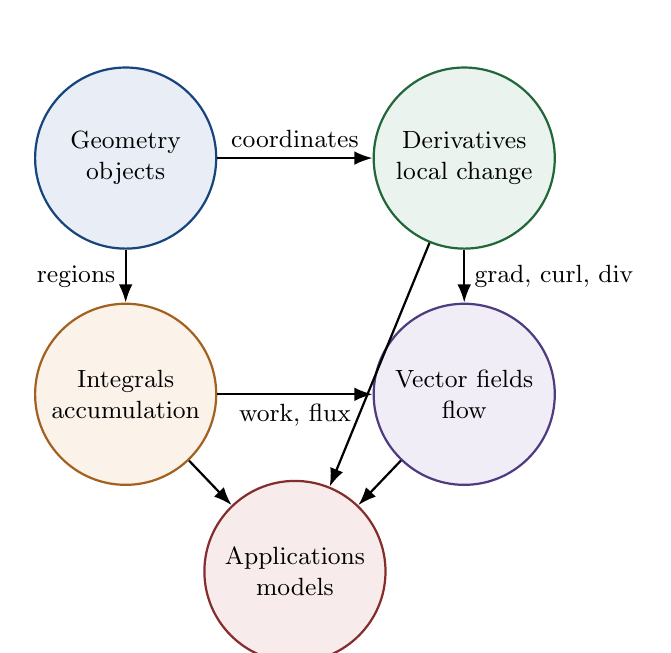
\begin{tikzpicture}[>=Latex, node distance=2.1cm, font=\small]
  \tikzset{topic/.style={circle, draw=#1!75!black, fill=#1!10, thick, minimum size=2.3cm, align=center}}
  \node[topic=chapterblue] (geo) at (0,1.4) {Geometry\\objects};
  \node[topic=chaptergreen] (der) at (4.3,1.4) {Derivatives\\local change};
  \node[topic=chapterorange] (int) at (0,-1.6) {Integrals\\accumulation};
  \node[topic=chapterpurple] (vf) at (4.3,-1.6) {Vector fields\\flow};
  \node[topic=chapterred] (app) at (2.15,-3.85) {Applications\\models};
  \draw[->,thick] (geo) -- node[above] {coordinates} (der);
  \draw[->,thick] (geo) -- node[left] {regions} (int);
  \draw[->,thick] (der) -- node[right] {grad, curl, div} (vf);
  \draw[->,thick] (int) -- node[below] {work, flux} (vf);
  \draw[->,thick] (der) -- (app);
  \draw[->,thick] (int) -- (app);
  \draw[->,thick] (vf) -- (app);
\end{tikzpicture}
\caption{A schematic map of the main objects in multivariable calculus.}
\end{figure}

\section*{27.2 Geometry: the coordinate language}

The first part of the book developed the coordinate language of space. The essential objects are points, vectors, distances, angles, projections, lines, planes, and surfaces. For $x=(x_1,\ldots,x_n)$ and $y=(y_1,\ldots,y_n)$,
\[
\norm{x-y}=\sqrt{(x_1-y_1)^2+\cdots+(x_n-y_n)^2}.
\]
The dot product is
\[
x\cdot y=x_1y_1+\cdots+x_ny_n,
\]
and it measures alignment:
\[
x\cdot y=\norm{x}\,\norm{y}\cos\theta.
\]
Projection is the geometry behind least squares and many data methods. The projection of $x$ onto the direction of a nonzero vector $v$ is
\[
\proj_v x=\frac{x\cdot v}{v\cdot v}v.
\]
A hyperplane in $\R^n$ has equation
\[
w\cdot x=b.
\]
This equation appears in tangent planes, constraints, regression, support vector machines, and linear classifiers.

\begin{examplebox}[Example 27.1: Projection as a least-squares approximation]
Let $x=(3,4)$ and $v=(1,2)$. The best approximation to $x$ among all multiples of $v$ is
\[
\proj_v x=\frac{x\cdot v}{v\cdot v}v=\frac{3+8}{1+4}(1,2)=\frac{11}{5}(1,2).
\]
The residual $r=x-\proj_v x$ is orthogonal to $v$. This is the same geometry used when fitting a linear model by least squares: the residual is orthogonal to the space of fitted values.
\end{examplebox}

\begin{figure}[H]
\centering
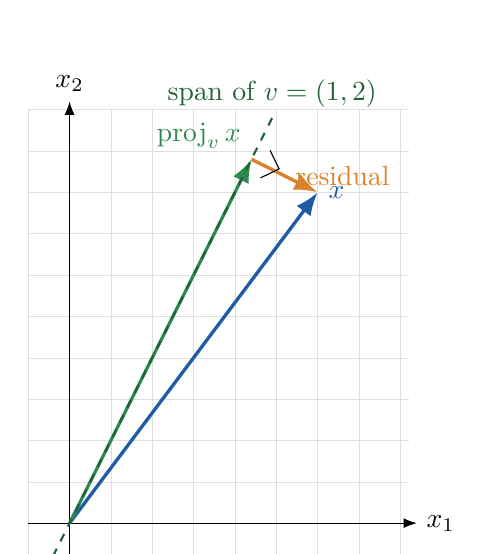
\begin{tikzpicture}[scale=1.05,>=Latex]
  \draw[help lines,step=0.5,gray!25] (-0.5,-0.5) grid (4.1,5.0);
  \draw[->] (-0.5,0) -- (4.2,0) node[right] {$x_1$};
  \draw[->] (0,-0.5) -- (0,5.1) node[above] {$x_2$};
  \coordinate (O) at (0,0);
  \coordinate (X) at (3,4);
  \coordinate (P) at (2.2,4.4);
  \draw[->,very thick,chapterblue] (O) -- (X) node[right] {$x$};
  \draw[->,very thick,chaptergreen] (O) -- (P) node[above left] {$\proj_v x$};
  \draw[->,very thick,chapterorange] (P) -- (X) node[midway,right] {residual};
  \draw[chaptergreen!70!black,thick,dashed] (-0.2,-0.4) -- (2.45,4.9) node[above] {span of $v=(1,2)$};
  \draw (2.2,4.4) ++(-64:0.25) -- ++(26:0.25) -- ++(116:0.25);
\end{tikzpicture}
\caption{Projection decomposes a vector into a component along a direction and an orthogonal residual.}
\end{figure}

\section*{27.3 Derivatives: local change and local models}

For a scalar function $f:\R^n\to\R$, the first derivative is the gradient
\[
\grad f(x)=\left(\frac{\partial f}{\partial x_1},\ldots,\frac{\partial f}{\partial x_n}\right).
\]
The gradient gives the best linear approximation, gives directional derivatives by dot product, and points in the direction of fastest increase. Near $a$,
\[
f(a+h)\approx f(a)+\grad f(a)\cdot h.
\]
The directional derivative in a unit direction $u$ is
\[
D_u f(a)=\grad f(a)\cdot u.
\]
The second derivative is organized by the Hessian matrix
\[
H_f(a)=
\begin{bmatrix}
\frac{\partial^2 f}{\partial x_1^2} & \cdots & \frac{\partial^2 f}{\partial x_1\partial x_n} \\
\vdots & \ddots & \vdots \\
\frac{\partial^2 f}{\partial x_n\partial x_1} & \cdots & \frac{\partial^2 f}{\partial x_n^2}
\end{bmatrix}.
\]
The second-order Taylor approximation is
\[
f(a+h)\approx f(a)+\grad f(a)\cdot h+\frac12 h^T H_f(a)h.
\]
This is the local geometry behind optimization, uncertainty approximation, and many algorithms in statistics and machine learning.

\begin{examplebox}[Example 27.2: Local quadratic geometry]
For $f(x,y)=x^2+4y^2$, we have $\grad f(0,0)=0$ and
\[
H_f(0,0)=\begin{bmatrix}2&0\\0&8\end{bmatrix}.
\]
The eigenvalues are positive, so the origin is a local minimum. The curvature is larger in the $y$-direction than in the $x$-direction.
\end{examplebox}

\begin{figure}[H]
\centering
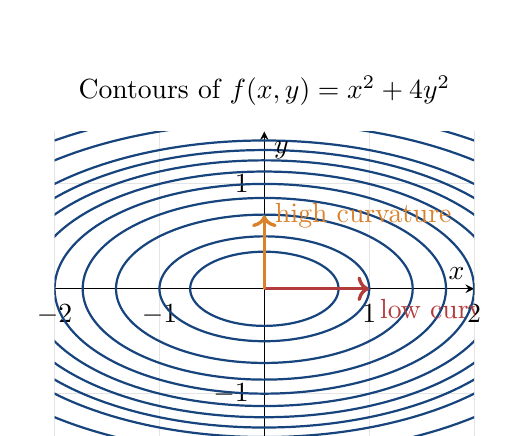
\begin{tikzpicture}
\begin{axis}[
  width=0.66\textwidth,
  height=0.46\textwidth,
  xmin=-2,xmax=2,ymin=-1.5,ymax=1.5,
  axis equal image,
  axis lines=middle,
  xlabel={$x$},ylabel={$y$},
  grid=both,
  major grid style={gray!20},
  title={Contours of $f(x,y)=x^2+4y^2$}
]
\foreach \c in {0.5,1,2,3,4,5,6,7,8,10,12,14,16}{
  \addplot[domain=0:360,samples=200,chapterblue!75!black,thick] ({sqrt(\c)*cos(x)},{sqrt(\c)/2*sin(x)});
}
\draw[->,very thick,chapterred] (axis cs:0,0) -- (axis cs:1,0) node[below right] {low curvature};
\draw[->,very thick,chapterorange] (axis cs:0,0) -- (axis cs:0,0.7) node[right] {high curvature};
\end{axis}
\end{tikzpicture}
\caption{A quadratic function is controlled by its Hessian matrix. Narrower contours correspond to larger curvature.}
\end{figure}

\section*{27.4 Jacobians: derivatives of vector-valued maps}

For a map $F:\R^n\to\R^m$, the derivative is the Jacobian matrix
\[
J_F(x)=
\begin{bmatrix}
\frac{\partial F_1}{\partial x_1} & \cdots & \frac{\partial F_1}{\partial x_n} \\
\vdots & \ddots & \vdots \\
\frac{\partial F_m}{\partial x_1} & \cdots & \frac{\partial F_m}{\partial x_n}
\end{bmatrix}.
\]
Near $a$,
\[
F(a+h)\approx F(a)+J_F(a)h.
\]
The Jacobian is the linear map used in the multivariable chain rule. If $F=G\circ H$, then
\[
J_F(x)=J_G(H(x))J_H(x).
\]
In computation, this is the matrix form of backpropagation. In integration, the determinant of the Jacobian measures how area or volume changes under a coordinate transformation.

\begin{examplebox}[Example 27.3: The polar-coordinate Jacobian]
The polar-coordinate map is
\[
T(r,\theta)=(r\cos\theta,r\sin\theta).
\]
Its Jacobian matrix is
\[
J_T(r,\theta)=
\begin{bmatrix}
\cos\theta & -r\sin\theta\\
\sin\theta & r\cos\theta
\end{bmatrix},
\qquad
|\det J_T(r,\theta)|=r.
\]
That is why $dA=r\,dr\,d\theta$.
\end{examplebox}

\begin{figure}[H]
\centering
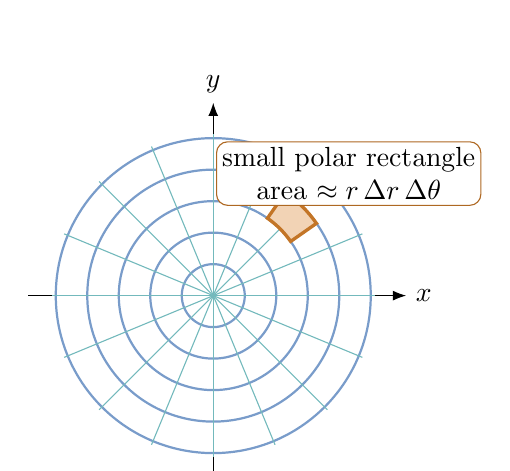
\begin{tikzpicture}[scale=1.0,>=Latex]
  \draw[->] (-2.35,0) -- (2.45,0) node[right] {$x$};
  \draw[->] (0,-2.35) -- (0,2.45) node[above] {$y$};
  \foreach \r in {0.4,0.8,1.2,1.6,2.0}{\draw[chapterblue!60,thick] (0,0) circle (\r);}
  \foreach \ang in {0,22.5,...,337.5}{\draw[chapterteal!60] (0,0) -- (\ang:2.05);}
  \fill[chapterorange!35] (35:1.2) arc (35:55:1.2) -- (55:1.6) arc (55:35:1.6) -- cycle;
  \draw[chapterorange!90!black,very thick] (35:1.2) arc (35:55:1.2) -- (55:1.6) arc (55:35:1.6) -- cycle;
  \node[align=center,fill=white,draw=chapterorange!80!black,rounded corners,inner sep=2pt] at (1.72,1.55) {small polar rectangle\\area $\approx r\,\Delta r\,\Delta\theta$};
\end{tikzpicture}
\caption{The polar-coordinate map stretches small rectangles by the Jacobian factor $r$.}
\end{figure}

\section*{27.5 Integrals: accumulation over geometric objects}

A definite integral accumulates over an interval. Multivariable calculus extends this idea to regions, solids, curves, and surfaces.

\begin{center}
\renewcommand{\arraystretch}{1.14}
\begin{tabularx}{\textwidth}{p{0.28\textwidth}p{0.22\textwidth}X}
\toprule
Integral & Object & Common meaning\\
\midrule
$\int_a^b f(x)\,dx$ & interval & signed area, total change\\
$\iint_R f(x,y)\,dA$ & plane region & volume, mass, probability\\
$\iiint_E f(x,y,z)\,dV$ & solid region & mass, volume, expectation\\
$\int_C f\,ds$ & curve & mass of a wire\\
$\int_C F\cdot dr$ & oriented curve & work, circulation\\
$\iint_S f\,dS$ & surface & mass of a shell\\
$\iint_S F\cdot n\,dS$ & oriented surface & flux\\
\bottomrule
\end{tabularx}
\end{center}

In statistics, integrals compute probability, expectation, variance, and normalization constants. In applied mathematics, integrals compute mass, energy, flow, and conservation quantities. In machine learning, integrals appear in expected risk, Bayesian inference, generative models, and continuous approximations.

\begin{examplebox}[Example 27.4: Probability as a double integral]
Suppose a joint density is
\[
f(x,y)=4xy,\qquad 0\le x\le 1,\quad 0\le y\le 1.
\]
Then $\iint_{[0,1]^2}4xy\,dA=1$, so it is a valid density. The probability of the event $x+y\le 1$ is
\[
\int_0^1\int_0^{1-x}4xy\,dy\,dx
=\int_0^1 2x(1-x)^2\,dx=\frac16.
\]
\end{examplebox}

\begin{figure}[H]
\centering
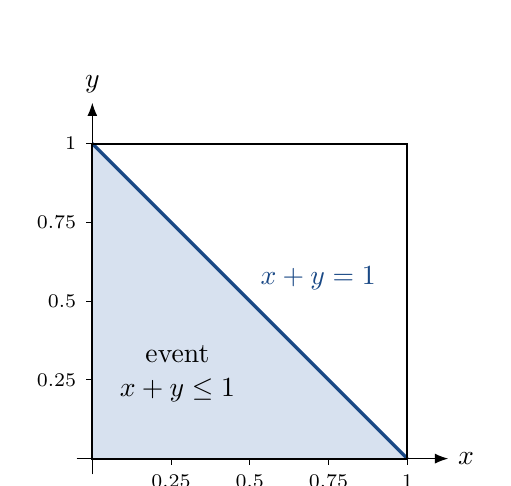
\begin{tikzpicture}[scale=4.0,>=Latex]
  \draw[->] (-0.05,0) -- (1.13,0) node[right] {$x$};
  \draw[->] (0,-0.05) -- (0,1.13) node[above] {$y$};
  \fill[chapterblue!18] (0,0) -- (1,0) -- (0,1) -- cycle;
  \draw[chapterblue!80!black,very thick] (0,1) -- (1,0) node[midway,above right] {$x+y=1$};
  \draw[thick] (0,0) rectangle (1,1);
  \foreach \x in {0.25,0.5,0.75,1}{\draw (\x,0) -- ++(0,-0.02) node[below,font=\scriptsize] {\x};}
  \foreach \y in {0.25,0.5,0.75,1}{\draw (0,\y) -- ++(-0.02,0) node[left,font=\scriptsize] {\y};}
  \node[align=center] at (0.27,0.27) {event\\$x+y\le 1$};
\end{tikzpicture}
\caption{A probability over a two-dimensional event is an integral over a region.}
\end{figure}

\section*{27.6 Optimization: from critical points to algorithms}

Optimization is one of the main bridges from calculus to data science and machine learning. The central objects are the gradient $\grad f$, the Hessian $H_f$, and constraint gradients $\grad g_i$.

For unconstrained optimization,
\[
\grad f(x)=0.
\]
For one constraint,
\[
\grad f(x)=\lambda \grad g(x),\qquad g(x)=c.
\]
For two constraints,
\[
\grad f(x)=\lambda \grad g(x)+\mu \grad h(x),\qquad g(x)=c,\quad h(x)=d.
\]
Gradient descent uses
\[
x_{k+1}=x_k-\alpha\grad f(x_k),
\]
while Newton's method uses curvature:
\[
x_{k+1}=x_k-H_f(x_k)^{-1}\grad f(x_k).
\]
The graduate-level habit is to ask not only where the optimum is, but also whether the problem is well-conditioned, whether the Hessian is positive definite, and whether constraints or regularization change the geometry.

\begin{figure}[H]
\centering
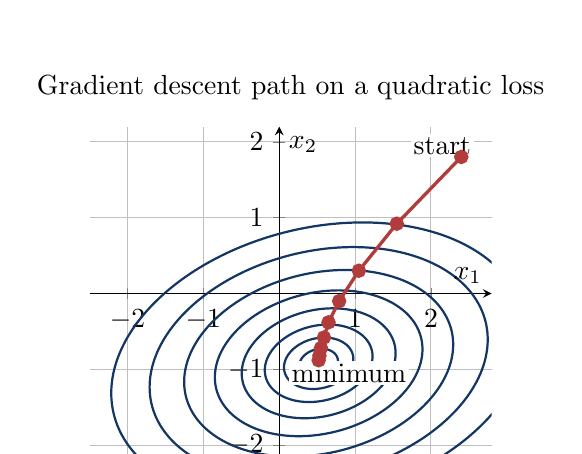
\begin{tikzpicture}
\begin{axis}[
  width=0.68\textwidth,height=0.48\textwidth,
  xmin=-2.5,xmax=2.8,ymin=-2.2,ymax=2.2,
  axis equal image,
  axis lines=middle,
  xlabel={$x_1$},ylabel={$x_2$},
  grid=both,
  title={Gradient descent path on a quadratic loss}
]
\foreach \a/\b in {0.25/0.18,0.45/0.32,0.7/0.48,1.0/0.68,1.35/0.9,1.75/1.15,2.2/1.43,2.7/1.73}{
  \addplot[domain=0:360,samples=180,chapterblue!60!black,thick] ({0.52 + \a*cos(x) - 0.25*\b*sin(x)},{-0.92 + 0.25*\a*cos(x) + \b*sin(x)});
}
\addplot[chapterred,very thick,mark=*] coordinates {(2.4,1.8) (1.55,0.92) (1.05,0.30) (0.79,-0.10) (0.65,-0.38) (0.59,-0.58) (0.55,-0.72) (0.53,-0.82) (0.52,-0.88)};
\node[fill=white,inner sep=1pt] at (axis cs:2.15,1.95) {start};
\node[fill=white,inner sep=1pt] at (axis cs:0.92,-1.05) {minimum};
\end{axis}
\end{tikzpicture}
\caption{Gradient descent follows local negative-gradient directions on a loss landscape.}
\end{figure}

\section*{27.7 Vector fields and the global theorems}

Vector calculus studies fields that assign a vector to each point. The main differential operators are
\[
\diver F=\grad\cdot F,
\qquad
\curl F=\grad\times F.
\]
Divergence measures local source or sink behavior. Curl measures local rotation. The global theorems convert integrals over boundaries into integrals over interiors.

\subsection*{The four Fundamental-Theorem patterns}

\begin{center}
\renewcommand{\arraystretch}{1.16}
\begin{tabularx}{\textwidth}{p{0.25\textwidth}p{0.24\textwidth}p{0.24\textwidth}X}
\toprule
Theorem & Boundary integral & Interior integral & Meaning\\
\midrule
FTC & $f(b)-f(a)$ & $\int_a^b f'(x)\,dx$ & endpoint change equals accumulated derivative\\
Line integral FTC & $f(B)-f(A)$ & $\int_C\grad f\cdot dr$ & potential difference equals work\\
Green's theorem & $\oint_C P\,dx+Q\,dy$ & $\iint_R(Q_x-P_y)\,dA$ & boundary circulation equals interior curl\\
Stokes theorem & $\oint_{\partial S}F\cdot dr$ & $\iint_S(\grad\times F)\cdot n\,dS$ & boundary circulation equals surface curl flux\\
Divergence theorem & $\iint_{\partial E}F\cdot n\,dS$ & $\iiint_E\grad\cdot F\,dV$ & boundary flux equals interior source\\
\bottomrule
\end{tabularx}
\end{center}
The pattern is powerful: a global boundary measurement is controlled by a local derivative inside.

\begin{figure}[H]
\centering
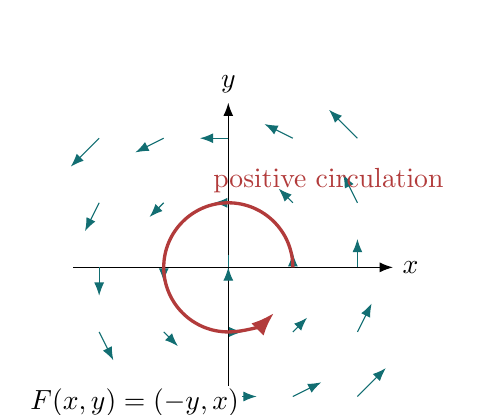
\begin{tikzpicture}[scale=0.82,>=Latex]
  \draw[->] (-2.4,0) -- (2.55,0) node[right] {$x$};
  \draw[->] (0,-2.4) -- (0,2.55) node[above] {$y$};
  \foreach \x in {-2,-1,0,1,2}{
    \foreach \y in {-2,-1,0,1,2}{
      \pgfmathsetmacro{\u}{-0.22*\y}
      \pgfmathsetmacro{\v}{0.22*\x}
      \draw[->,chapterteal!80!black] (\x,\y) -- ++(\u,\v);
    }
  }
  \draw[chapterred,very thick,->] (1,0) arc (0:315:1);
  \node[chapterred] at (1.55,1.35) {positive circulation};
  \node[fill=white,inner sep=1pt] at (-1.45,-2.1) {$F(x,y)=(-y,x)$};
\end{tikzpicture}
\caption{A rotational vector field illustrates circulation around closed curves.}
\end{figure}

\section*{27.8 A problem-solving decision tree}

A good problem-solving strategy is often more useful than a memorized formula.

\begin{figure}[H]
\centering
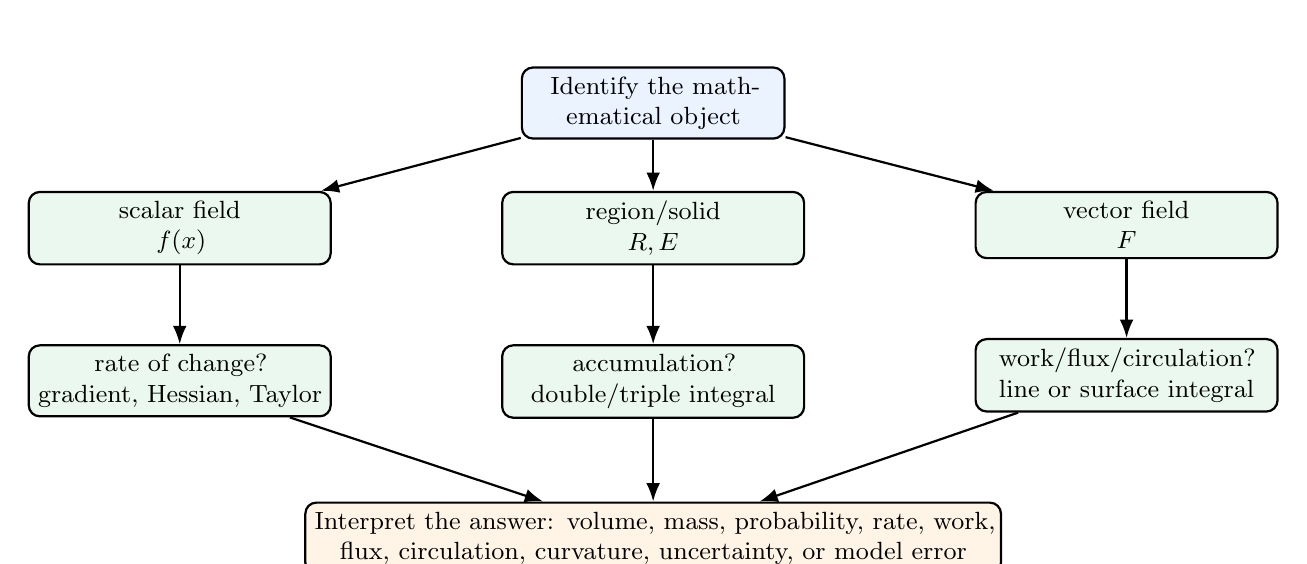
\begin{tikzpicture}[>=Latex,node distance=1.15cm,font=\small]
\tikzset{box/.style={draw,rounded corners,align=center,thick,minimum height=0.65cm,text width=3.1cm,fill=softblue}}
\tikzset{act/.style={draw,rounded corners,align=center,thick,minimum height=0.58cm,text width=3.6cm,fill=softgreen}}
\node[box] (start) {Identify the mathematical object};
\node[act,below left=0.65cm and 2.4cm of start] (scalar) {scalar field\\$f(x)$};
\node[act,below=0.65cm of start] (region) {region/solid\\$R,E$};
\node[act,below right=0.65cm and 2.4cm of start] (field) {vector field\\$F$};
\node[act,below=1.0cm of scalar] (deriv) {rate of change?\\gradient, Hessian, Taylor};
\node[act,below=1.0cm of region] (intg) {accumulation?\\double/triple integral};
\node[act,below=1.0cm of field] (flow) {work/flux/circulation?\\line or surface integral};
\node[box,fill=softorange,below=1.05cm of intg,text width=8.6cm] (interpret) {Interpret the answer: volume, mass, probability, rate, work, flux, circulation, curvature, uncertainty, or model error};
\draw[->,thick] (start) -- (scalar);
\draw[->,thick] (start) -- (region);
\draw[->,thick] (start) -- (field);
\draw[->,thick] (scalar) -- (deriv);
\draw[->,thick] (region) -- (intg);
\draw[->,thick] (field) -- (flow);
\draw[->,thick] (deriv) -- (interpret);
\draw[->,thick] (intg) -- (interpret);
\draw[->,thick] (flow) -- (interpret);
\end{tikzpicture}
\caption{Decision tree: identify the object, identify the action, then interpret the result.}
\end{figure}

\section*{27.9 A compact formula sheet with meaning}

\begin{formulabox}[Derivatives]
\[
D_u f(a)=\grad f(a)\cdot u,\quad \norm{u}=1,
\qquad
f(a+h)\approx f(a)+\grad f(a)\cdot h,
\]
\[
f(a+h)\approx f(a)+\grad f(a)\cdot h+\frac12 h^T H_f(a)h,
\qquad
J_{G\circ F}(x)=J_G(F(x))J_F(x).
\]
\end{formulabox}

\begin{formulabox}[Optimization]
\[
\grad f=0,
\qquad
\grad f=\lambda\grad g,
\qquad
x_{k+1}=x_k-\alpha\grad f(x_k).
\]
\end{formulabox}

\begin{formulabox}[Multiple integrals and coordinate factors]
\[
\iint_R f(x,y)\,dA,
\qquad
\iiint_E f(x,y,z)\,dV,
\]
\[
dA=r\,dr\,d\theta,
\qquad
dV=r\,dr\,d\theta\,dz,
\qquad
dV=\rho^2\sin\phi\,d\rho\,d\phi\,d\theta.
\]
\end{formulabox}

\begin{formulabox}[Vector calculus]
\[
\int_C F\cdot dr,
\qquad
\iint_S F\cdot n\,dS,
\qquad
\grad\cdot F,
\qquad
\grad\times F.
\]
\[
\oint_{\partial R}P\,dx+Q\,dy=\iint_R(Q_x-P_y)\,dA,
\]
\[
\oint_{\partial S}F\cdot dr=\iint_S(\grad\times F)\cdot n\,dS,
\qquad
\iint_{\partial E}F\cdot n\,dS=\iiint_E\grad\cdot F\,dV.
\]
\end{formulabox}

\section*{27.10 Computational capstone: a mini calculus toolkit}

This section builds a small numerical toolkit. The goal is not to replace exact mathematics, but to make the formulas executable. A graduate student should be able to move between exact formulas, numerical approximations, and visual checks.

\begin{figure}[H]
\centering
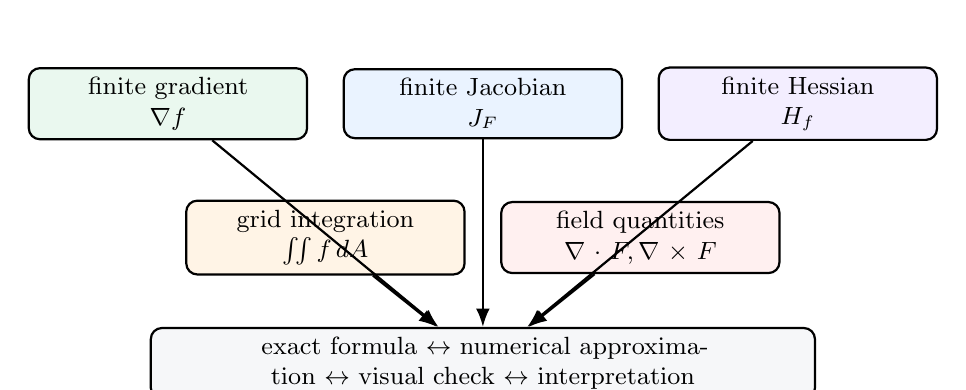
\begin{tikzpicture}[>=Latex,font=\small]
\tikzset{tool/.style={draw,rounded corners,thick,align=center,minimum height=0.72cm,text width=3.3cm}}
\node[tool,fill=softgreen] (grad) at (0,1.7) {finite gradient\\$\nabla f$};
\node[tool,fill=softblue] (jac) at (4.0,1.7) {finite Jacobian\\$J_F$};
\node[tool,fill=softpurple] (hess) at (8.0,1.7) {finite Hessian\\$H_f$};
\node[tool,fill=softorange] (integ) at (2.0,0) {grid integration\\$\iint f\,dA$};
\node[tool,fill=softred] (curl) at (6.0,0) {field quantities\\$\nabla\cdot F,\nabla\times F$};
\node[draw,rounded corners,thick,fill=softgray,align=center,text width=8.2cm,minimum height=0.78cm] (interp) at (4,-1.6) {exact formula $\leftrightarrow$ numerical approximation $\leftrightarrow$ visual check $\leftrightarrow$ interpretation};
\foreach \a in {grad,jac,hess,integ,curl}{\draw[->,thick] (\a) -- (interp);}
\end{tikzpicture}
\caption{A mini calculus toolkit turns derivative and integral formulas into executable approximations.}
\end{figure}

\begin{lstlisting}[style=pythonstyle,caption={Finite differences for gradients and Hessians.}]
def finite_gradient(f, x, h=1e-6):
    g = zeros_like(x)
    for j in range(len(x)):
        e = coordinate_vector(j)
        g[j] = (f(x + h*e) - f(x - h*e))/(2*h)
    return g

def finite_hessian(f, x, h=1e-4):
    H = zeros((len(x), len(x)))
    for i in range(len(x)):
        for j in range(len(x)):
            H[i,j] = centered_second_difference(f, x, i, j, h)
    return H
\end{lstlisting}

\begin{figure}[H]
\centering
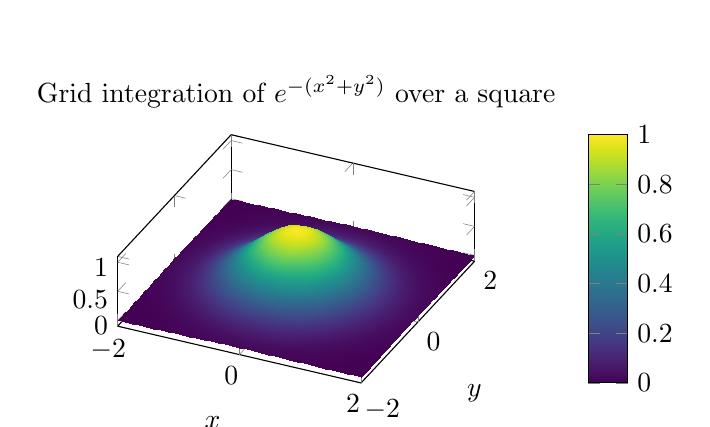
\begin{tikzpicture}
\begin{axis}[
  width=0.66\textwidth,height=0.46\textwidth,
  xmin=-2,xmax=2,ymin=-2,ymax=2,
  axis equal image,
  xlabel={$x$},ylabel={$y$},
  title={Grid integration of $e^{-(x^2+y^2)}$ over a square},
  colorbar,
  colormap/viridis
]
\addplot3[surf,domain=-2:2,y domain=-2:2,samples=35,samples y=35,shader=interp] {exp(-(x^2+y^2))};
\end{axis}
\end{tikzpicture}
\caption{Grid integration approximates accumulation over a rectangle.}
\end{figure}

\begin{warningbox}[Numerical computation is not proof]
A numerical approximation can suggest a pattern, check an answer, or make a concept visible. It does not replace a proof. In graduate work, the best habit is to combine computation with exact reasoning: use computation to explore, and use mathematics to explain.
\end{warningbox}

\section*{27.11 Graduate-study bridge}

The following table shows how the main ideas of this book reappear in later courses.

\begin{center}
\renewcommand{\arraystretch}{1.12}
\begin{tabularx}{\textwidth}{>{\bfseries}p{0.27\textwidth}X}
\toprule
Later area & Multivariable calculus foundation\\
\midrule
Real analysis & limits, continuity, differentiability, rigorous approximation\\
Linear algebra & vector spaces, projections, hyperplanes, quadratic forms\\
Optimization & gradients, Hessians, convexity, constraints, descent methods\\
Probability & joint densities, transformations, expectation, covariance\\
Mathematical statistics & likelihood, score, Hessian, Fisher information, delta method\\
Machine learning & loss functions, backpropagation, gradient descent, regularization\\
Numerical analysis & finite differences, numerical integration, error analysis\\
Differential equations & vector fields, gradient flow, divergence, curl, conservation laws\\
Partial differential equations & gradient, divergence, Laplacian, flux, boundary conditions\\
Geometry and topology & curves, surfaces, orientation, Stokes-type theorems\\
\bottomrule
\end{tabularx}
\end{center}

The most important preparation is not memorizing every formula. It is learning how to translate a new problem into the correct mathematical object.

\section*{27.12 Capstone project: build a calculus engine}

A strong final project for this book is to build a small package or notebook called \texttt{calculus\_engine}. It should include:
\begin{enumerate}
  \item \texttt{finite\_gradient(f, x)}
  \item \texttt{finite\_jacobian(F, x)}
  \item \texttt{finite\_hessian(f, x)}
  \item \texttt{integrate\_rectangle(f, xlim, ylim)}
  \item \texttt{monte\_carlo\_integral(f, sampler)}
  \item \texttt{line\_integral(F, r, a, b)}
  \item \texttt{surface\_flux(F, r, u\_range, v\_range)}
  \item \texttt{gradient\_descent(f, grad, x0, alpha)}
  \item \texttt{newton\_step(f, grad, hessian, x)}
  \item \texttt{plot\_contours(f)}
\end{enumerate}
The project should include examples from probability, optimization, and vector calculus, together with written interpretations of each output.

\subsection*{Example project theme: one dataset, many calculus ideas}
Choose a simple dataset with input-output pairs $(x_i,y_i)$. Fit a linear regression model
\[
\hat y_i=\beta_0+\beta_1x_i.
\]
Then study the least-squares loss
\[
L(\beta_0,\beta_1)=\sum_{i=1}^n(y_i-\beta_0-\beta_1x_i)^2.
\]
This one example uses vectors for data, a scalar field for the loss landscape, gradients for optimization, Hessians for curvature, contour plots for visualization, linear approximation for sensitivity, and probability if errors are modeled as random noise.

\begin{figure}[H]
\centering
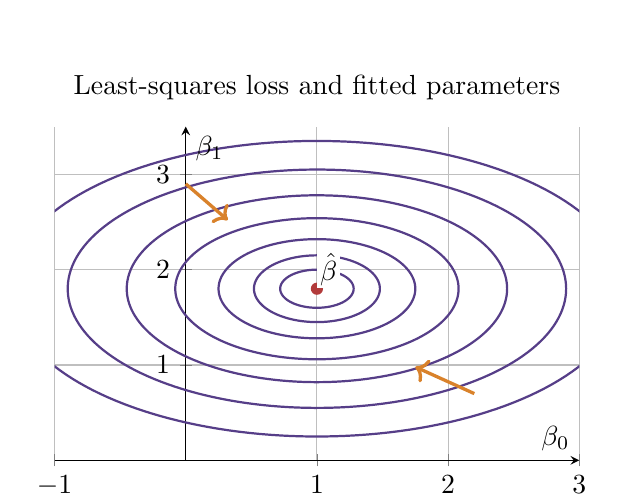
\begin{tikzpicture}
\begin{axis}[
  width=0.68\textwidth,height=0.48\textwidth,
  xmin=-1,xmax=3,ymin=0,ymax=3.5,
  axis lines=middle,
  xlabel={$\beta_0$},ylabel={$\beta_1$},
  grid=both,
  title={Least-squares loss and fitted parameters}
]
\foreach \a/\b in {0.28/0.20,0.48/0.35,0.75/0.52,1.08/0.74,1.45/0.98,1.9/1.25,2.35/1.55}{
  \addplot[domain=0:360,samples=180,chapterpurple!80!black,thick] ({1.0+\a*cos(x)},{1.8+\b*sin(x)});
}
\fill[chapterred] (axis cs:1.0,1.8) circle (2.2pt);
\node[above right,fill=white,inner sep=1pt] at (axis cs:1.0,1.8) {$\hat\beta$};
\draw[->,very thick,chapterorange] (axis cs:2.2,0.7) -- (axis cs:1.75,0.98);
\draw[->,very thick,chapterorange] (axis cs:0.0,2.9) -- (axis cs:0.32,2.52);
\end{axis}
\end{tikzpicture}
\caption{A single least-squares loss landscape connects vectors, gradients, Hessians, optimization, and statistics.}
\end{figure}

\section*{27.13 Common mistakes to avoid}

\begin{enumerate}
  \item \textbf{Confusing points and vectors.} A point gives location; a vector gives displacement. Coordinates can represent either, but the meaning differs.
  \item \textbf{Forgetting that multivariable limits require all paths.} Checking one path is not enough to prove a limit exists.
  \item \textbf{Using the gradient without normalizing the direction.} Directional derivatives use unit vectors.
  \item \textbf{Forgetting boundary cases in optimization.} Critical points inside a region are not enough for absolute extrema.
  \item \textbf{Missing the Jacobian factor.} Coordinate changes require area or volume scaling.
  \item \textbf{Using the wrong orientation.} Line and surface integrals over oriented objects depend on direction.
  \item \textbf{Applying Green, Stokes, or Divergence theorem without checking hypotheses.} Holes, singularities, and missing boundaries matter.
  \item \textbf{Treating numerical output as exact.} Computation supports reasoning but does not replace it.
\end{enumerate}

\section*{27.14 Cumulative worked example}

\begin{examplebox}[A single field using many tools]
Consider
\[
f(x,y)=x^2+xy+2y^2.
\]
The gradient is
\[
\grad f(x,y)=(2x+y,x+4y),
\qquad
\grad f(1,-1)=(1,-3).
\]
In the unit direction $u=\frac{1}{\sqrt5}(1,2)$,
\[
D_u f(1,-1)=(1,-3)\cdot\frac{1}{\sqrt5}(1,2)=-\sqrt5.
\]
The Hessian is
\[
H_f=\begin{bmatrix}2&1\\1&4\end{bmatrix}.
\]
It is positive definite because its leading principal minors are positive. Therefore $f$ is strictly convex and has a unique global minimum where $\grad f=0$, namely $(0,0)$.

The average value over $[-1,1]\times[-1,1]$ is
\[
\frac{1}{4}\int_{-1}^1\int_{-1}^1(x^2+xy+2y^2)\,dy\,dx.
\]
By symmetry, the $xy$ term integrates to zero, so the average is
\[
\frac14\left(\frac43+\frac83\right)=1.
\]
This one example uses gradients, directional derivatives, Hessians, optimization, symmetry, and double integrals.
\end{examplebox}

\begin{figure}[H]
\centering
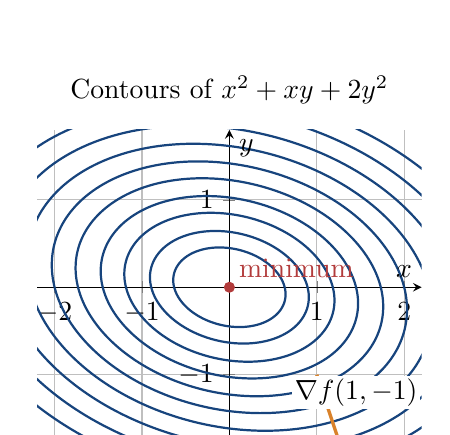
\begin{tikzpicture}
\begin{axis}[
  width=0.66\textwidth,height=0.46\textwidth,
  xmin=-2.2,xmax=2.2,ymin=-1.8,ymax=1.8,
  axis equal image,
  axis lines=middle,
  xlabel={$x$},ylabel={$y$},
  grid=both,
  title={Contours of $x^2+xy+2y^2$}
]
\foreach \c in {0.4,0.8,1.4,2.1,3,4,5.2,6.6,8.2,10}{
  \addplot[domain=0:360,samples=220,chapterblue!75!black,thick] ({sqrt(\c)*cos(x)-0.18*sqrt(\c)*sin(x)},{0.72*sqrt(\c)*sin(x)});
}
\fill[chapterred] (axis cs:0,0) circle (2pt) node[above right] {minimum};
\addplot[chapterorange,very thick,-Latex] coordinates {(1,-1) (1.55,-2.65)};
\node[fill=white,inner sep=1pt] at (axis cs:1.45,-1.2) {$\nabla f(1,-1)$};
\end{axis}
\end{tikzpicture}
\caption{The cumulative example combines contour geometry, gradients, Hessians, and optimization.}
\end{figure}

\section*{27.15 Practice problems}

\subsection*{Conceptual review}
\begin{enumerate}
  \item Explain the difference between a scalar field and a vector field. Give one example of each.
  \item Explain why the gradient is perpendicular to level curves.
  \item Explain the difference between a double integral over a region and a line integral over a curve.
  \item Explain why the Jacobian determinant appears in change of variables.
  \item Compare Green's theorem, Stokes theorem, and the Divergence theorem in one paragraph.
\end{enumerate}

\subsection*{Core skills}
\begin{enumerate}[start=6]
  \item Let $f(x,y)=x^2+3xy+y^2$. Compute $\grad f$, $H_f$, and the directional derivative at $(1,2)$ in the direction $(3,4)$.
  \item Find the tangent plane to $z=x^2+y^2$ at $(1,2,5)$.
  \item Compute $\iint_R xy\,dA$, where $R=[0,2]\times[1,3]$.
  \item Change $\int_0^1\int_y^1 e^{x^2}\,dx\,dy$ to the opposite order.
  \item Use polar coordinates to evaluate $\iint_R(x^2+y^2)\,dA$, where $R$ is the disk $x^2+y^2\le 4$.
\end{enumerate}

\subsection*{Vector calculus}
\begin{enumerate}[start=11]
  \item For $F(x,y)=(-y,x)$, compute $\oint_C F\cdot dr$ where $C$ is the unit circle oriented counterclockwise.
  \item For $F(x,y,z)=(x,y,z)$, compute the flux through the sphere $x^2+y^2+z^2=a^2$ using the Divergence theorem.
  \item Find a potential function for $F(x,y)=(2xy,x^2+3y^2)$ if one exists.
  \item Compute $\grad\cdot F$ and $\grad\times F$ for $F(x,y,z)=(yz,xz,xy)$.
\end{enumerate}

\subsection*{Statistics, data science, and applied mathematics}
\begin{enumerate}[start=15]
  \item Let $L(\beta_0,\beta_1)=\sum_{i=1}^n(y_i-\beta_0-\beta_1x_i)^2$. Derive the gradient of $L$.
  \item Let $f(x,y)=ce^{-(x^2+y^2)}$. Find $c$ so that $f$ is a probability density on $\R^2$.
  \item For a differentiable loss function $L(\theta)$, explain how the Hessian near a minimum is related to curvature and uncertainty.
  \item Write pseudocode for gradient descent and explain the role of the step size.
  \item Explain why a conservation law naturally involves divergence.
  \item Design one computational experiment that illustrates a major theorem from vector calculus.
\end{enumerate}

\section*{27.16 Python lab and interactive page}

\begin{itemize}
  \item Notebook lab: \texttt{Chapter27\_Review\_Synthesis\_and\_Bridge\_to\_Graduate\_Study.ipynb}
  \item Interactive HTML page: \path{../htmls/chapter-27.html}
\end{itemize}

\section*{Chapter summary}

\begin{summarybox}[Final synthesis]
This chapter organized multivariable calculus as a coherent language for modern quantitative work. Geometry describes the spaces and objects. Derivatives describe local change. Integrals describe accumulation. Optimization turns derivatives into algorithms. Vector calculus connects local field behavior with global boundary behavior. Probability and statistics reinterpret integrals as probabilities and expectations, and machine learning reinterprets gradients and Hessians as tools for fitting models.

The deepest lesson is that the same mathematical structures appear across many subjects. A tangent plane, a linear approximation, a least-squares projection, a gradient descent step, a probability density, a flux integral, and a conservation law are not isolated facts. They are connected parts of one multivariable calculus language.
\end{summarybox}

\end{document}
